\section{GPU Architecture and Concepts}\label{gpu}
%--------------------------------------------------------------------------------------
\subsection{Parallelism}\label{gpu:sec:par}
One of the main means of optimizing processing is through parallelism. The two main forms of parallelism are task and data parallelism. Task parallelism can be seen as running multiple processes concurrently where communication between the processes is explicitly defined to avoid race conditions. Data parallelism is the distribution of a data set over a number of identical processes each of which performs operations on a unique subset of the data. Race conditions occur when parallel processing streams access data or perform operations out of the intended order, leading to errors or incorrect output being produced. A combination of task and data parallelism can lead to an ideal speed-up, but both have their limits depending on the task and the data being operated on (\cite{subhlok1993exploiting}).
\\
\\
The increased need for parallelism came in about 2005, when CPU frequency peaked at 4 GHz due to heat dissipation issues. However, Moore's Law still holds, and is still expected to hold until 2025; that is, that the number of transistors for a computer will double every two years. This leads to a problem where the speed at which an operation is done cannot be increased (due to the frequency limit), but the number of concurrent operations can still increase. This means that the only way to speed up an operation is to change it from a sequential to a parallel process (\cite{rajan2013informatics}).
%--------------------------------------------------------------------------------------
\subsection{GPU Optimization}\label{gpu:sec:opt}
GPU's were originally designed for rendering pixels and vectors in games. They were especially designed for this since CPU's are optimized to run sequential instructions as fast as possible; whereas pixel and vector calculations are inherently parallel. With NVIDIA's release of CUDA in 2006, general purpose GPU (GPGPU) programming became common place as a way to accelerate data processing through data parallelism and task parallelism through the simultaneous execution of similar task (\cite{nvidia_cuda}).
\\
\\
The power of GPU's come from its architecture which is optimized for a special case of SIMD (Single Instruction Multiple Data) processing known as SIMT (Single Instruction Multiple Threads). SIMD allows a central processor to distribute a set of instructions to multiple simple processors which then act on the data simultaneously. SIMT is more generalized as each thread of the GPU can perform different tasks given the same set of instructions. This is due to the way in which the GPU handles branching at the thread level. By exploiting these processes, and this instructional architecture, some instructions can be computed in faster time than that of a CPU (\cite{vuduc2013brief}).
%--------------------------------------------------------------------------------------
\subsection{The NVIDIA GeForce GTX 750 Ti}\label{gpu:sec:750}
%
\subsubsection{GM107 Maxwell Architecture}\label{gpu:ssec:max}
The NVIDIA GeForce GTX 750 Ti GPU was released on the 18th of February 2014. It boasts 640 CUDA cores, 1020 MHz base clock speed, 1305.6 GFLOPs and a memory bandwidth of 86.4 GB/sec. It is NVIDIA's first-generation Maxwell architecture, designed for high performance at relatively low power consumption (60 W) and has the codename 'GM107'. The GPU uses PCI Express 3.0 to interface with the host machine through the GigaThread engine. The first-generation Maxwell (from now simply referred to as Maxwell) is made up of one Graphics Processing Cluster (GPC) on which the processing occurs. It also contains a large L2 cache at 2048 KB and two 64-bit memory controllers to access the 2048 MB global memory. This design can be seen in Figure \ref{gpu:img:gm107} (\cite{geforce_750}, \cite{g750_specs}, \cite{g750_paper}).
%
\subsubsection{Streaming Multiprocessors}\label{gpu:ssec:smm}
The GPC is further broken down into five Streaming Multiprocessors(SM) which are further divided into four processing blocks. The processing blocks each contain an instruction buffer, a scheduler and 32 CUDA cores as seen in Figure \ref{gpu:img:smm} (\cite{GM107SMM}). These warps are set in a lock step, meaning each core in a warp executes the same command, with different valued variable.
%
\begin{figure}[H]
 \centering
 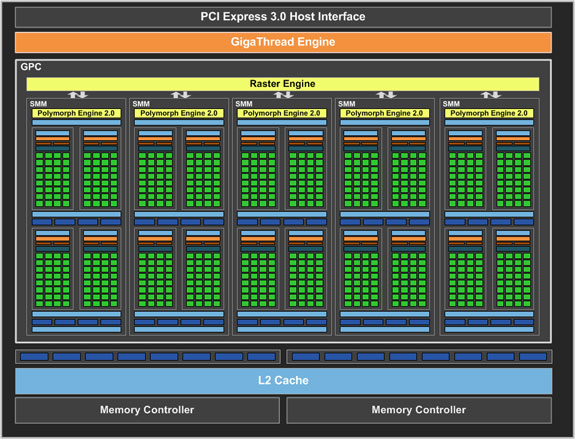
\includegraphics[width=0.7\textwidth]{Images/GM107.jpg}
 \caption{NVIDIA Maxwell Architecture\cite{GM107}}
 \label{gpu:img:gm107}
\end{figure}
%
\begin{figure}[H]
\centering
 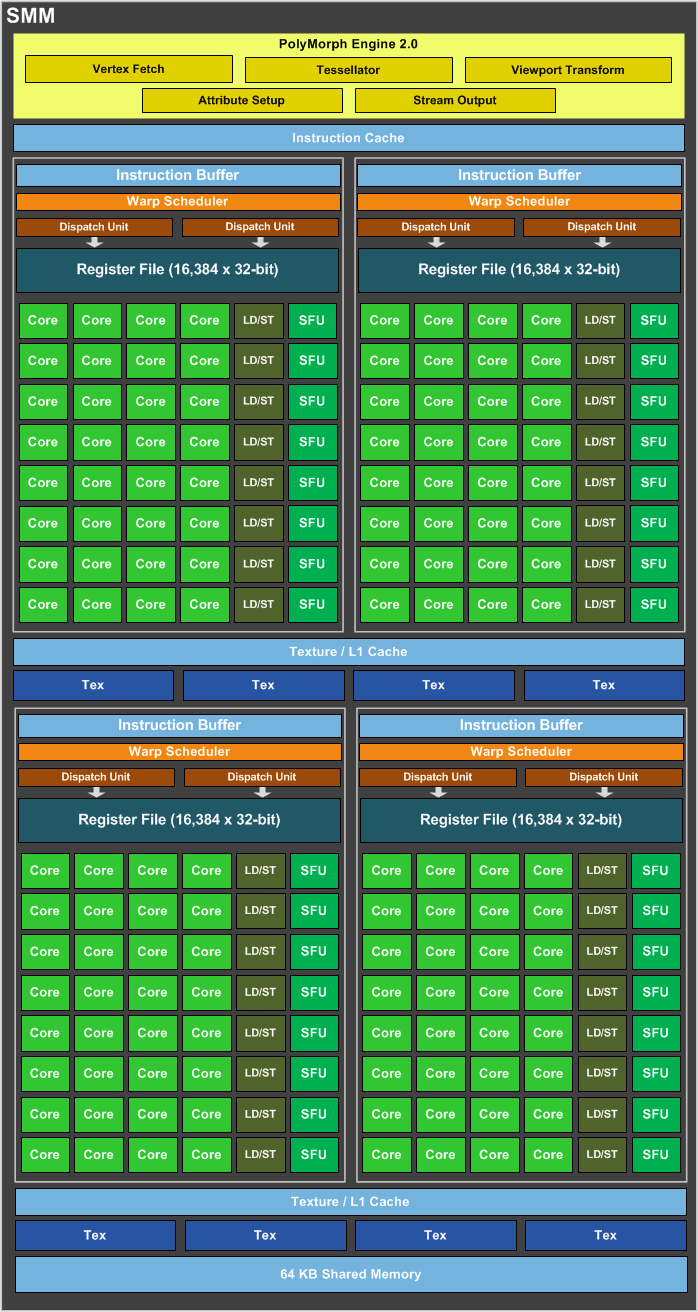
\includegraphics[width=0.4\textwidth]{Images/GM107SMM.png}
 \caption{Maxwell Streaming Multiprocessor\cite{GM107SMM}}
 \label{gpu:img:smm}
\end{figure}
%--------------------------------------------------------------------------------------
\subsection{GPU Memory}\label{gpu:sec:mem}
%
\subsubsection{Registry Memory}\label{gpu:ssec:reg}
%
\subsubsection{Cache}\label{gpu:ssec:cache}
%
\subsubsection{Global Memory}\label{gpu:ssec:gm}
%
\subsubsection{Constant Memory}\label{gpu:ssec:cm}
%--------------------------------------------------------------------------------------
